\documentclass[10pt,a4paper]{article}
\usepackage[a4paper, total={6.5in, 9in}]{geometry}
\usepackage[latin1]{inputenc}
\usepackage{amsmath}
\usepackage{amsfonts}
\usepackage{amssymb}
\usepackage{mathtools}
\usepackage{graphicx}
\usepackage{float}
\usepackage[usenames, dvipsnames]{color}
\usepackage{fancyhdr}
\usepackage{enumitem}
\usepackage{listings}
\usepackage{siunitx}
\setlength{\headheight}{15.2pt}
\pagestyle{fancy}
\setlength{\parindent}{0em}
\setlength{\parskip}{10pt}
\setlist[enumerate,1]{label=\alph*)}
\setlist[enumerate,2]{label=(\roman*)}
\definecolor{LGray}{gray}{0.9}
\definecolor{deepgreen}{rgb}{0,0.5,0}
\lstset{language=python, tabsize=4, breaklines=true, postbreak=\mbox{\textcolor{red}{$\hookrightarrow$}\space}, basicstyle=\linespread{0.7}\ttfamily, commentstyle=\color{deepgreen},} 
\newcommand*\diff{\mathop{}\!\mathrm{d}}



\begin{document}
\title{COMP90086 Assignment 3}
\author{Benjamin Cheng-Hsien Yi}
\rhead{Benjamin Cheng-Hsien Yi - 1152795}
\lhead{COMP90086 Assignment 3}

\section{Methodology}

\subsection*{Finding keypoints and correspondences}
SIFT from the cv2 module was used to compute keypoints in both images. FLANN (a knn algorithm) from the cv2 module was then used to match keypoints to determine correspondences. At this point, a findHomography, another cv2 module was used to calculate inliers for visualisation purposes - no data was from this function otherwise, apart from obtaining an initial estimate of inlier rate.

Note that much of this step's code was derived from workshops 7 and 8.

\subsection*{Shifting and scaling pixel co-ordinates}
When calculating the fundamental matrix, a poorly distributed set of correspondence points across the image co-ordinate domain may lead to an ill-defined null space and therefore an inaccurate fundamental matrix. To counteract this, correspondence point co-ordinates are shifted and scaled to be centered at (0, 0) and have average distance of sqrt(2) from the origin.

This was achieved by constructing a transformation matrix T defined as:

\begin{equation}
	T = 
	\begin{bmatrix}
		s & 0 & 0\\
		0 & s & 0\\
		0 & 0 & 1
	\end{bmatrix}
	\times
	\begin{bmatrix}
		1 & 0 & -xc\\
		0 & 1 & -yc\\
		0 & 0 & 1
	\end{bmatrix}
\end{equation}

where s is the scale factor, and xc, yc are centroids of the correspondence points. The new pixel co-ordinates are then calculated as $x_{new} = Tx$ for each co-ordinate point.

\subsection*{Computing design matrix}
Eight random points were chosen from all correspondence points. The reason to use only 8 points is because it is the minimum to form the fundamental matrix, and using more would only increase the computation time taken to find a fundamental matrix free of outliers. The design matrix was formed thus:

\begin{equation}
	\begin{bmatrix}
		p_1^{(1)}q_1^{(1)} & p_2^{(1)}q_1^{(1)} & q_1^{(1)} & p_1^{(1)}q_2^{(1)} & p_2^{(1)}q_2^{(1)} & q_2^{(1)} & p_1^{(1)} & p_2^{(1)} & 1\\
		p_1^{(2)}q_1^{(2)} & p_2^{(2)}q_1^{(2)} & q_1^{(2)} & p_1^{(2)}q_2^{(2)} & p_2^{(2)}q_2^{(2)} & q_2^{(2)} & p_1^{(2)} & p_2^{(2)} & 1\\
		\vdots & \vdots & \vdots & \vdots & \vdots & \vdots & \vdots & \vdots & \vdots\\
		p_1^{(n)}q_1^{(n)} & p_2^{(n)}q_1^{(n)} & q_1^{(n)} & p_1^{(n)}q_2^{(n)} & p_2^{(n)}q_2^{(n)} & q_2^{(n)} & p_1^{(n)} & p_2^{(n)} & 1
	\end{bmatrix}
\end{equation}

where $p^{(n)}$ refers to the co-ordinates of the nth corresponding point in the left image, and $q^{(n)}$ to the right.

\subsection*{Performing SVD on the design matrix}
Numpy's svd function is used to perform SVD on the design matrix, returning $A=UDV$ where A is the design matrix.

\subsection*{Composing F}
To find the fundamental matrix, the final column from $V$ was extracted. As numpy's svd function returns results in decreasing order of magnitude, the least singular value is always from the final column. The fundamental matrix is simply the final column re-arranged into a 3x3 matrix.

\subsection*{Performing SVD on F}
SVD is performed on F, setting the last row of $D$ to zero and reassembling. This has the effect of changing the determinant of F to zero, making it a rank-2 matrix. This is important to reduce the effects of noisy image co-ordinates, which may cause the definition $q^TDp = 0$ to fail.

\subsection*{Calculating inliers}
The first step is to calculate epilines. To find the epilines for the left image (right image follows similarly):
\begin{equation}
	a, b, c = F_uq_n
\end{equation}
where:
\begin{equation}
	ax + by + c = 0
\end{equation}
F is unscaled and unshifted back to image co-ordinates by applying:
\begin{equation}
	F_u = T_R^T \times F \times T_L
\end{equation}
where $T_R$ is the translation matrix from the right image and $T_L$ is the translation matrix from the left image.

The distance from each point to their epiline is then calculated thus:
\begin{equation}
	d =
	\begin{bmatrix}
		a_R & b_R & c_R
	\end{bmatrix}
	\times 
	F
	\times
	\begin{bmatrix}
		a_L \\
		b_L \\
		c_L
	\end{bmatrix}
\end{equation}

Whie inliners should theoretically lie upon their epilines exactly, numerical error leads to slight distances so an error tolerance of 1e-3 was used as the distance cutoff for inliner identification.

\subsection*{RANSAC loop}
The above steps were wrapped into a RANSAC loop, randomly choosing 8 correspondence points to form the design matrix each time. The RANSAC loop was ran for 5000 iterations. The iteration number was chosen by the process below:

First, initial inlier rate estimates were collected from the first step. Inlier rates varied from 5\% to 80\% depending on the images. Then the iteration count required to have 99\% confidence of finding 8 inliers was then calculated from:

\begin{equation}
	\frac{\log(1 - 0.99)}{\log(1 - r^8)}
\end{equation}

where $r$ was the inlier rate for that image.

As some images required absurd amounts of iterations to form 99\% confidence, I manually chose a value of 5000 iterations that satisfied the majority of non-absurd iteration counts. This strikes a balance between obtaining 99\% confidence for most images with considerations of run-time becoming untenable.

The iteration which yielded the highest amount of inliers was then chosen as the output fundamental matrix.

\subsection*{Re-estimate F}
Finally, one more iteration was ran, using all inliers from the output fundamental matrix as part of the design matrix to return the final high-quality fundamental matrix.

\subsection*{Re-compute F}
The final fundamental matrix was then unscaled and unshifted back to the original pixel co-ordinates thus:
\begin{equation}
	F_u = T_R^T \times F \times T_L
\end{equation}
similar to previously when calculating inliers.

\newpage
\section{Results}
File: booksh\\
Calculated number of iterations needed: 17656\\
Fundamental matrix:
\begin{figure}[H]
	\centering
	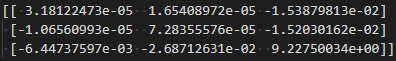
\includegraphics[width=0.7\linewidth]{img/bookshf}
	\caption{booksh fundamental matrix}
	\label{fig:bookshf}
\end{figure}
\begin{figure}[H]
	\centering
	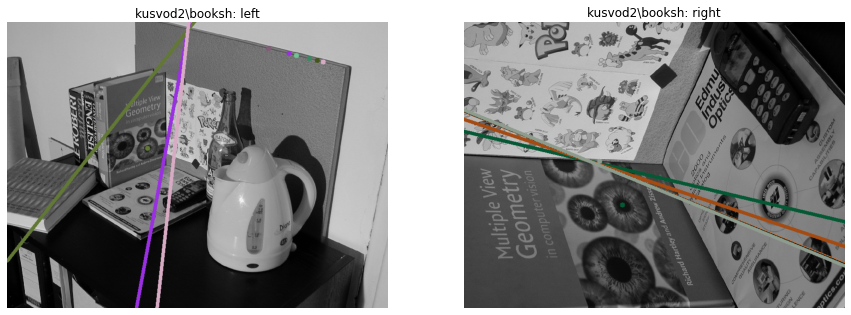
\includegraphics[width=0.7\linewidth]{img/booksh}
	\caption{booksh epilines and inliers}
	\label{fig:booksh}
\end{figure}

File: box\\
Calculated number of iterations needed: 323\\
Fundamental matrix:
\begin{figure}[H]
	\centering
	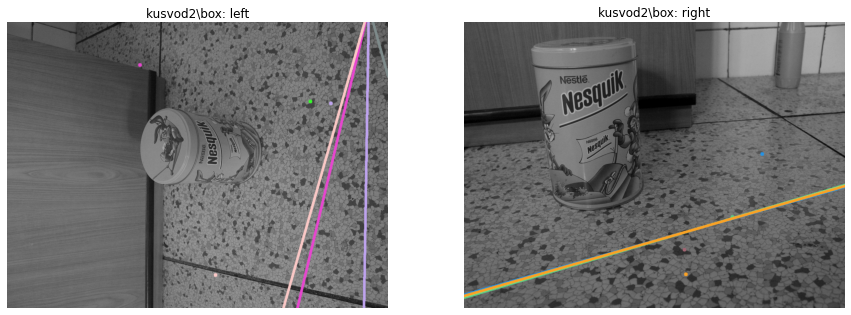
\includegraphics[width=0.7\linewidth]{img/box}
	\caption{box epilines and inliers}
	\label{fig:box}
\end{figure}

File: castle\\
Calculated number of iterations needed: 2436\\
Fundamental matrix:
\begin{figure}[H]
	\centering
	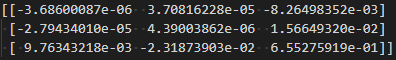
\includegraphics[width=0.7\linewidth]{img/castlef}
	\caption{castle fundamental matrix}
	\label{fig:castlef}
\end{figure}
\begin{figure}[H]
	\centering
	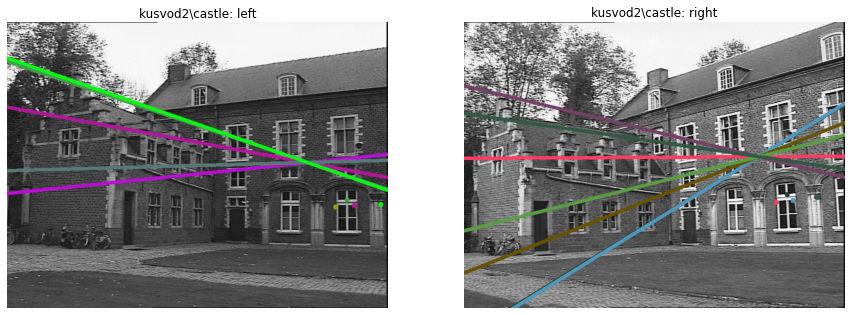
\includegraphics[width=0.7\linewidth]{img/castle}
	\caption{castle epilines and inliers}
	\label{fig:castle}
\end{figure}

File: corr\\
Calculated number of iterations needed: 21\\
Fundamental matrix:
\begin{figure}[H]
	\centering
	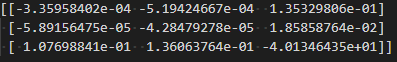
\includegraphics[width=0.7\linewidth]{img/corrf}
	\caption{corr fundamental matrix}
	\label{fig:corrf}
\end{figure}
\begin{figure}[H]
	\centering
	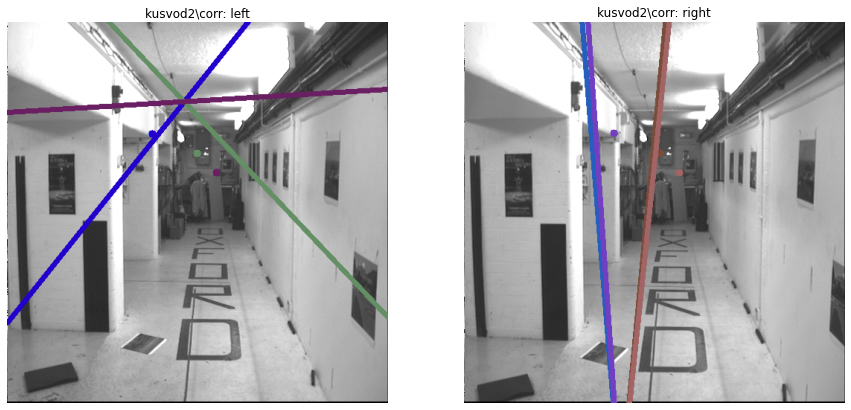
\includegraphics[width=0.7\linewidth]{img/corr}
	\caption{corr epilines and inliers}
	\label{fig:corr}
\end{figure}

File: graff\\
Calculated number of iterations needed: 333684762580\\
Fundamental matrix:
\begin{figure}[H]
	\centering
	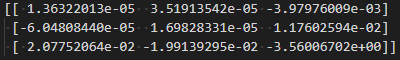
\includegraphics[width=0.7\linewidth]{img/grafff}
	\caption{graff fundamental matrix}
	\label{fig:grafff}
\end{figure}
\begin{figure}[H]
	\centering
	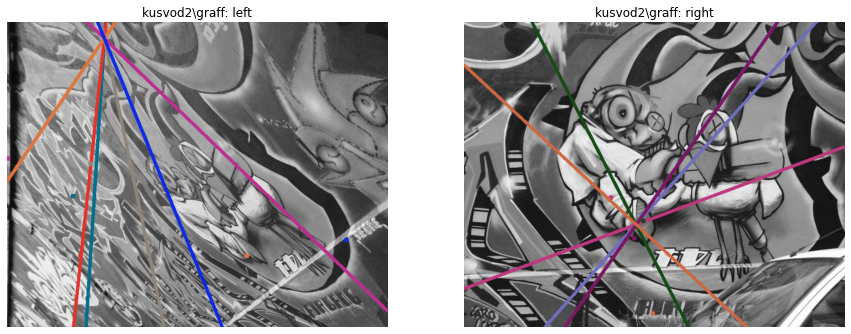
\includegraphics[width=0.7\linewidth]{img/graff}
	\caption{graff epilines and inliers}
	\label{fig:graff}
\end{figure}

File: head\\
Calculated number of iterations needed: 361900\\
Fundamental matrix:
\begin{figure}[H]
	\centering
	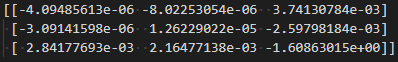
\includegraphics[width=0.7\linewidth]{img/headf}
	\caption{head fundamental matrix}
	\label{fig:headf}
\end{figure}
\begin{figure}[H]
	\centering
	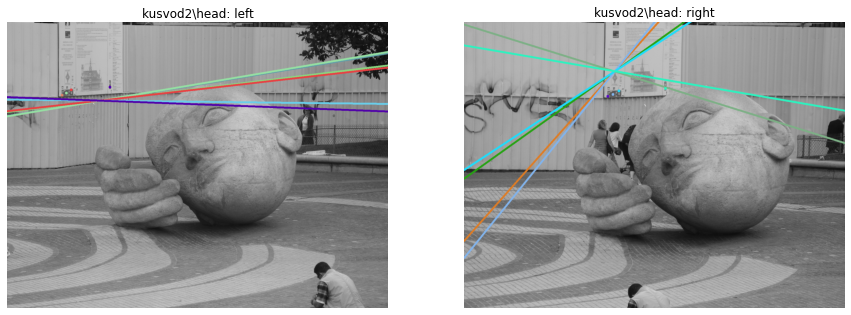
\includegraphics[width=0.7\linewidth]{img/head}
	\caption{head epilines and inliers}
	\label{fig:head}
\end{figure}

File: kampa\\
Calculated number of iterations needed: 3484\\
Fundamental matrix:
\begin{figure}[H]
	\centering
	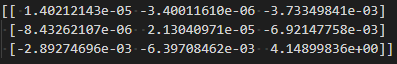
\includegraphics[width=0.7\linewidth]{img/kampaf}
	\caption{kampa fundamental matrix}
	\label{fig:kampaf}
\end{figure}
\begin{figure}[H]
	\centering
	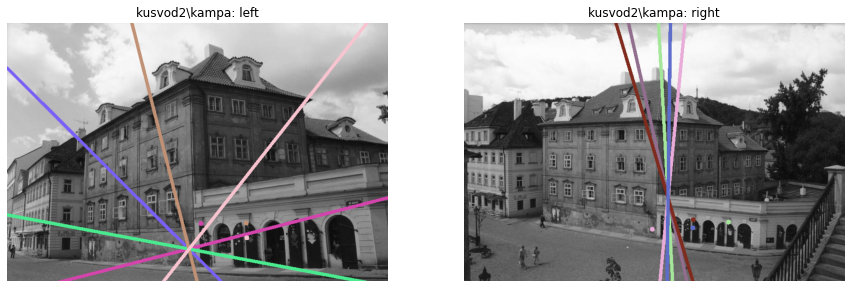
\includegraphics[width=0.7\linewidth]{img/kampa}
	\caption{kampa epilines and inliers}
	\label{fig:kampa}
\end{figure}

File: Kyoto\\
Calculated number of iterations needed: 451255715\\
Fundamental matrix:
\begin{figure}[H]
	\centering
	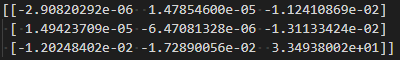
\includegraphics[width=0.7\linewidth]{img/Kyotof}
	\caption{Kyoto fundamental matrix}
	\label{fig:Kyotof}
\end{figure}
\begin{figure}[H]
	\centering
	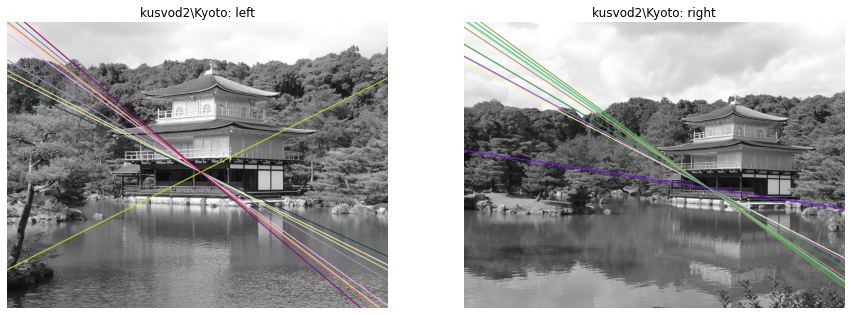
\includegraphics[width=0.7\linewidth]{img/Kyoto}
	\caption{Kyoto epilines and inliers}
	\label{fig:Kyoto}
\end{figure}

File: leafs\\
Calculated number of iterations needed: 54232373972\\
Fundamental matrix:
\begin{figure}[H]
	\centering
	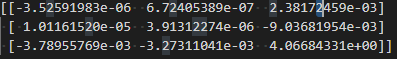
\includegraphics[width=0.7\linewidth]{img/leafsf}
	\caption{leafs fundamental matrix}
	\label{fig:leafsf}
\end{figure}
\begin{figure}[H]
	\centering
	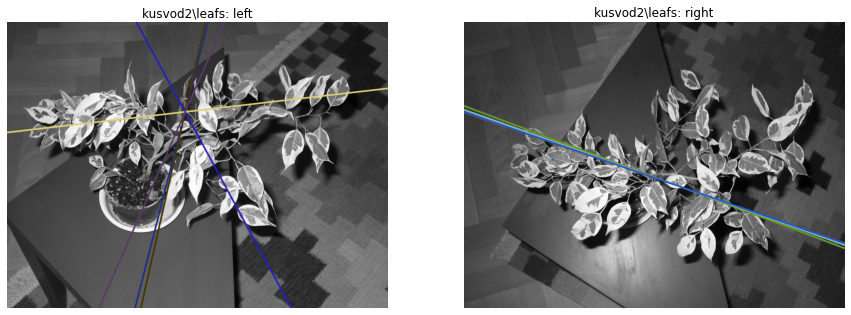
\includegraphics[width=0.7\linewidth]{img/leafs}
	\caption{leafs epilines and inliers}
	\label{fig:leafs}
\end{figure}

File: plant\\
Calculated number of iterations needed: 155610550\\
Fundamental matrix:
\begin{figure}[H]
	\centering
	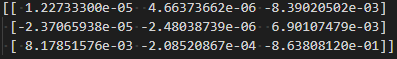
\includegraphics[width=0.7\linewidth]{img/plantf}
	\caption{plant fundamental matrix}
	\label{fig:plantf}
\end{figure}
\begin{figure}[H]
	\centering
	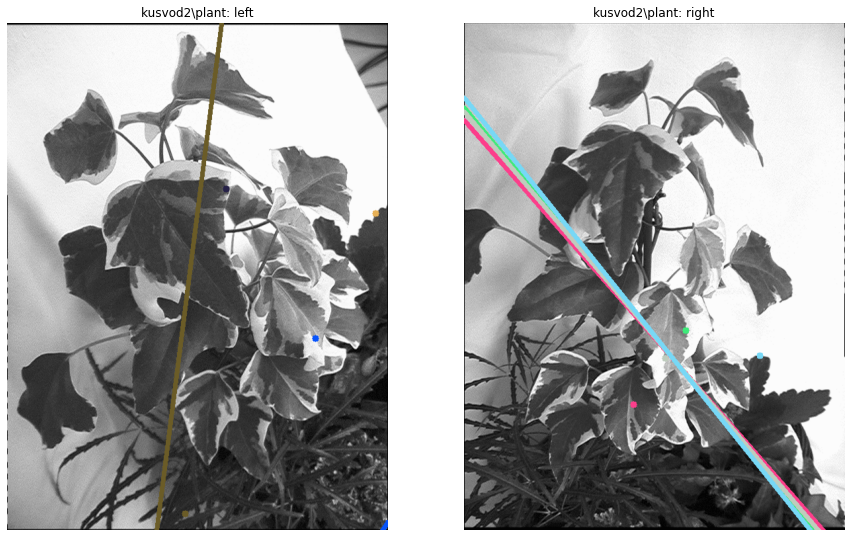
\includegraphics[width=0.7\linewidth]{img/plant}
	\caption{plant epilines and inliers}
	\label{fig:plant}
\end{figure}

File: rotunda\\
Calculated number of iterations needed: 941216\\
Fundamental matrix:
\begin{figure}[H]
	\centering
	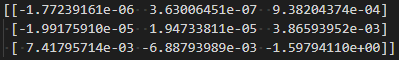
\includegraphics[width=0.7\linewidth]{img/rotundaf}
	\caption{rotunda fundamental matrix}
	\label{fig:rotundaf}
\end{figure}
\begin{figure}[H]
	\centering
	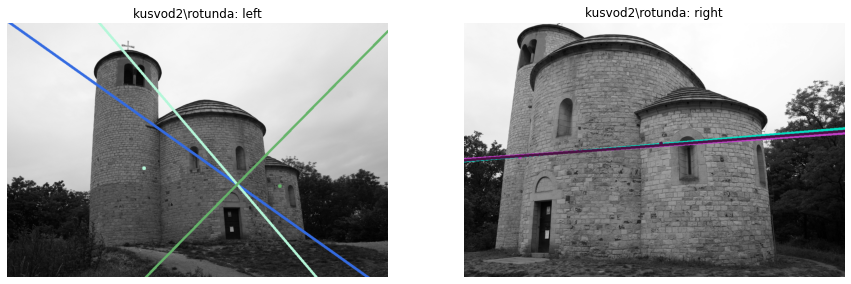
\includegraphics[width=0.7\linewidth]{img/rotunda}
	\caption{rotunda epilines and inliers}
	\label{fig:rotunda}
\end{figure}

File: shout\\
Calculated number of iterations needed: 6569\\
Fundamental matrix:
\begin{figure}[H]
	\centering
	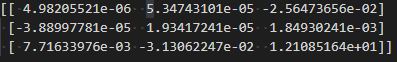
\includegraphics[width=0.7\linewidth]{img/shoutf}
	\caption{shout fundamental matrix}
	\label{fig:shoutf}
\end{figure}
\begin{figure}[H]
	\centering
	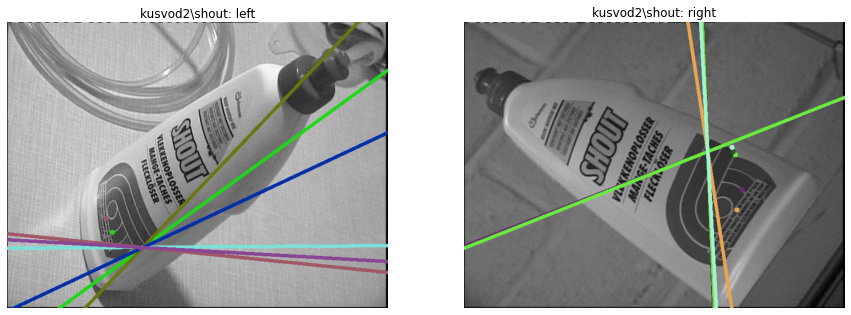
\includegraphics[width=0.7\linewidth]{img/shout}
	\caption{shout epilines and inliers}
	\label{fig:shout}
\end{figure}

File: valbonne\\
Calculated number of iterations needed: 489\\
Fundamental matrix:
\begin{figure}[H]
	\centering
	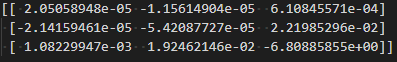
\includegraphics[width=0.7\linewidth]{img/valbonnef}
	\caption{valbonne fundamental matrix}
	\label{fig:valbonnef}
\end{figure}
\begin{figure}[H]
	\centering
	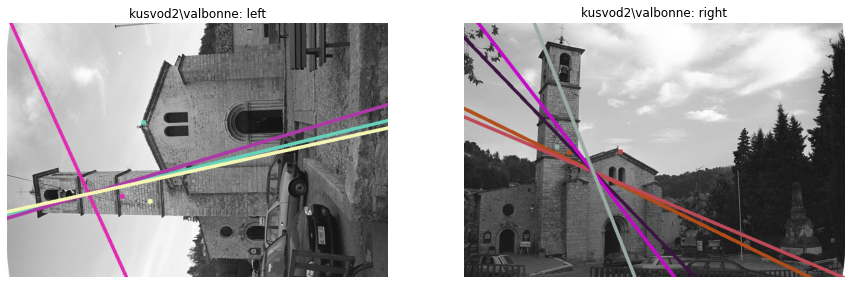
\includegraphics[width=0.7\linewidth]{img/valbonne}
	\caption{valbonne epilines and inliers}
	\label{fig:valbonne}
\end{figure}

File: wall\\
Calculated number of iterations needed: 172695723\\
Fundamental matrix:
\begin{figure}[H]
	\centering
	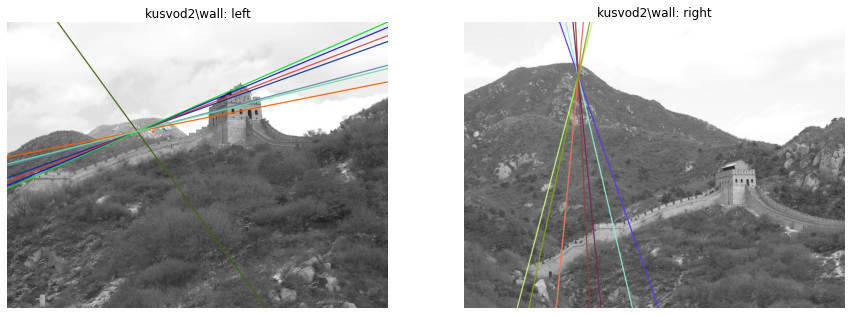
\includegraphics[width=0.7\linewidth]{img/wall}
	\caption{wall fundamental matrix}
	\label{fig:wallf}
\end{figure}
\begin{figure}[H]
	\centering
	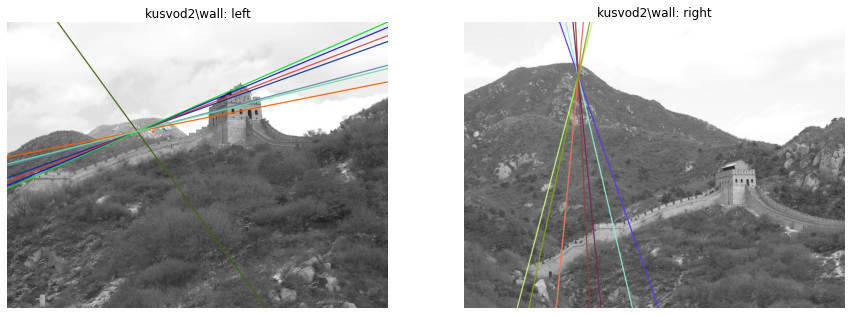
\includegraphics[width=0.7\linewidth]{img/wall}
	\caption{wall epilines and inliers}
	\label{fig:wall}
\end{figure}

File: wash\\
Calculated number of iterations needed: 2591030\\
Fundamental matrix:
\begin{figure}[H]
	\centering
	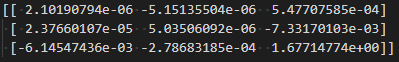
\includegraphics[width=0.7\linewidth]{img/washf}
	\caption{wash fundamental matrix}
	\label{fig:washf}
\end{figure}
\begin{figure}[H]
	\centering
	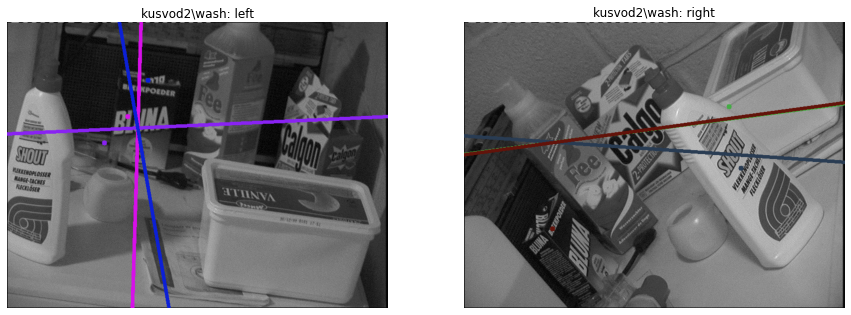
\includegraphics[width=0.7\linewidth]{img/wash}
	\caption{wash epilines and inliers}
	\label{fig:wash}
\end{figure}

File: zoom\\
Calculated number of iterations needed: 23240\\
Fundamental matrix:
\begin{figure}[H]
	\centering
	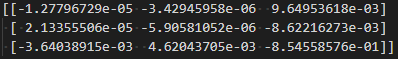
\includegraphics[width=0.7\linewidth]{img/zoomf}
	\caption{zoom fundamental matrix}
	\label{fig:zoomf}
\end{figure}
\begin{figure}[H]
	\centering
	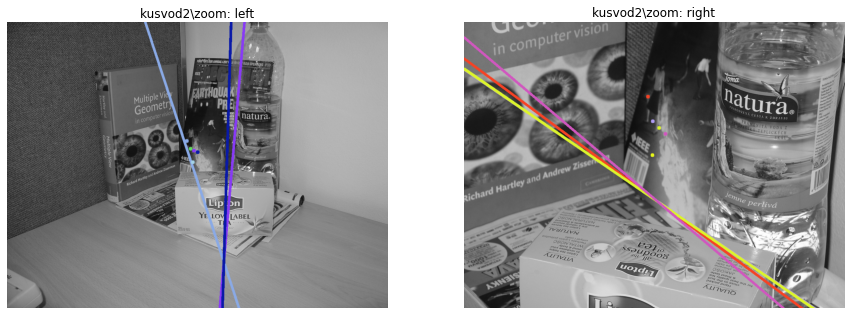
\includegraphics[width=0.7\linewidth]{img/zoom}
	\caption{zoom epilines and inliers}
	\label{fig:zoom}
\end{figure}

\newpage
\section{Discussion}
Clearly the fundamental matrices calculated are of low quality and the epilines drawn in the images are of dubious accuracy. This is possibly due to an insufficient number of iterations ran for the RANSAC loops due to time constraints. However, more likely is a mistake in step 1, with finding correspondences which then propagated to the final results. This is evident due to the incredibly absurd iteration counts calculated from inlier rates. Another possibility is errors in the fundamental matrix calculations.

Regardless, images "box", "graff", "plant", and "wall" seemed to be most difficult to analyse.\\
Image "box" contains a complicated table surface pattern which may have confused the correspondence calculations, leading to inaccurate correspondences.\\
Image "graff" consists of two very different angles, so the extreme angle difference may have lead to difficulty in calculating correspondences again.\\
Image "plant" has difficult to identify edges.\\
Image "wall" seems to have an entire mountain visible in the right image which is missing in the left image, along with other missing features from both sides, leading to many false positives in correspondence point analysis.

\end{document}

